\sloppy
\section{Life Cycle}
\begin{figure}[ht]
	\centerline{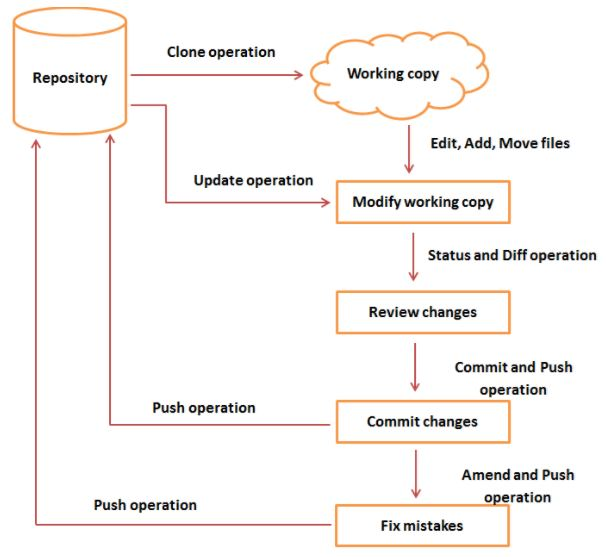
\includegraphics[width=0.25\textwidth]{Figures/git_life_cycle}}
	\caption{Life Cycle}
	\label{lifecycle}
\end{figure}
\vspace{12pt}
\noindent 
Git adalah sebuah perangkat lunak untuk mengontrol versi sebuah perangkat lunak "VCS/Version Control System". Git diciptakan oleh Linux Torvalds, yang pada awalnya ditujukan untuk pengembangan kernel Linux. Saat ini banyak perangkat lunak yang terkenal menggunakan Git sebagai pengotrol revisinya. \par
\vspace{12pt}
\noindent 
Pada tutorial ini Anda akan mempelajari bagaimana cara menggunakan Git seperti proses life cycle Git, operasi-operasi dasar dan bagaimana cara menangani masalah saat menggunakan Git. \par
\vspace{12pt}
\noindent 
Activity life cycle adalah sebuah siklus kehidupan activity. Sangat penting untuk memahami activity lifecyle ini untuk menghindari kebocoran memory. Dengan mengimplementasikan activity lifecyle ini kita bisa mengoptimalkan perfoma dari aplikasi yang kita buat. Setidaknya ada 6 siklus activity yang perlu kita pelajari, yaitu $  $onCreate, onStart, onResume onPause, onStop, dan onDestroy.
\begin{enumerate}
	\item onCreate OnCreate adalah state pada saat sebuah halaman atau activity pertama kali di buat atau di atach kedakam memory. OnCreate ini hanya di jalankan pada saat pertama kali di buat, jika sebuah acivity telah tersedia dalam backstact oncreate ini tidak di panggil lagi.
	\item onStart OnStart adalah state setelah oncreate di jalankan. OnStart juga tetap di jalankan walaupun oncreate tidak di panggil dengan sarat sebuah activity telah tersimpan di dalam backstact memory. OnStart ini juga di jalankan jika masih berada dalam state onStop.
	\item onResume OnResume di eksekusi setelah on start. OnResume ini di jalankan jika kita memanggil onPause.
	\item onPause OnPause ini setelah onResume. Ketika onPause ini di jalankan activity sudah dalam keadaan hilang atau sudah tidak tampil di user interface.
	\item onStop OnStop ini di akses setelah on pause dan sebelum aktivity ini benar - benar di hapus dari memory.
	\item onDestroy OnDestroy adalah bagian terakhir ketika activity benar - benar di hapus dari memory. Ketika sebuah activity telah di destroy maka tidak bisa melakukan onResume atau onStart.
\end{enumerate}
   

\subsection{SQLite Database}
\vspace{12pt}
\noindent 
SQLite adalah salah satu portable database yang bisa kita gunakan untuk menyimpan data sesuai dengan kebutuhan aplikasi yang kita buat. Ada beberapa lite database yang bisa di gunakan dalam pembuatan aplikasi android. Namun SQLite database ini adalah yang ada secara default yang tersedia di android. Untuk SQLite ini juga menggunakan query yang cukup mirip - mirip dengan MYSQL. Jadi jika sudah terbiasa dengan MYSQL maka tidak akan kesulitan untuk memulai menggunakan SQLite ini. \par
\vspace{12pt}
\noindent 
Content Provider \par
\vspace{12pt}
\noindent 
Content Provider adalah sebuah facilitas di android untuk kita gunakan untuk mengatur akses ke satu set terstruktur data. Dengan Content Provider memungkinkan kita untuk bisa share data dengan aplikasi lain. \par
\begin{enumerate}
	\item Determine URI's
	\item Update Contract
	\item Fill Out our URI matcher
	\item Implemen Function
\end{enumerate}


  
\vspace{12pt}
\vspace{12pt}
\vspace{12pt}
\noindent 
Sebagian dari anda mungkin sering bercengkerama dengan yang namanya komputer. Terutama para programmer, apalagi yang masih jomblo. Kasihan ya, yang dibuat cengkrama keseharian cuma komputer, server, dan kroni-kroninya.. hehe :p. Saya doakan deh para jomblo-jomblo yang belum menikah, semoga diberi jalan dan kemudahan Oleh Allah Subhanahu Wa Ta’ala untuk segera menemukan dambaan hatinya..aamiin \par
\noindent 
Kembali ke laptop, di tutorial kali ini saya akan membagikan materi tentang pengenalan GIT. Ini adalah salah satu bagian dari materi pelatihan git dan gitlab di kantor Telkomsel di Jakarta. Pelatihan ini adalah ini atas permintaan dari pihak Telkomsel untuk membagikan pengalaman penggunaan GIT dan GITLAB, terutama ketika di implementasikan dalam pengembangan project-project sistem yang sering di pegang oleh Profio Teknova Indonesia. Memang semenjak awal kami berdiri, hampir 2 tahun lalu, kami langsung menerapkan sistem kerja menggunakan Repository(GIT). Terbukti ini adalah formula yang cukup ampuh ketika kita melakukan development project secara bersama – sama. \par
\vspace{12pt}
\noindent 
Git adalah tools yang berfungsi sebagai Version Control System (VCS) pelacak perubahan pada file. Git sendiri dibuat oleh orang yang menciptakan Kernel Linux., yah mungkin temen-temen sudah kenal nama linus torvalds ya.. dialah Pencetus git, yang kita gunakan. Git diciptakan tahun 2005 saat bitkeeper mulai retak dan pencipta linux harus mencari alternatif lain untuk mendukung pengembangan kernel linux. Dengan menggunakan Git, setiap orang dalam sebuah tim dapat melakukan perubahan pada source-code tanpa harus takut terjadi bentrok ataupun kesulitan dalam menggabungkan hasil perubahan yang mereka lakukan. \par
\noindent 
\vspace{\baselineskip}
Dengan menggunakan Git, setiap perubahan pada source-code akan terlacak pesan perubahannya, apa saja yang diubah, siapa yang mengubah dan kapan waktunya. \par
\vspace{12pt}
\noindent 
Langsung saja, kita coba berkenalan dengan perintah – perintah dasar yang sering digunakan ketika bekerja menggunakan sistem repository: \par
\vspace{12pt}
\noindent 
git init $  $ \par
\noindent 
\vspace{\baselineskip}
Untuk membuat repo lokal baru pada perintah ini akan dibuat sebuah folder baru yang bernama  $ " $.git $ " $ \par
\noindent 
\vspace{\baselineskip}
\begin{verbatim}
 $ git init
\end{verbatim}
\begin{verbatim}
$ git status
\end{verbatim}
\vspace{\baselineskip}
untuk melihat status dari repo local \par
\noindent 
\vspace{\baselineskip}
Contoh : masuk ke direktori repo local \par
\noindent 
\vspace{\baselineskip}
 $  \$  $ git status \par
\vspace{12pt}
\noindent 
git add $  $ \par
\noindent 
\vspace{\baselineskip}
Untuk menambahkan file ke dalam repo yang sebelumnya sudah dibuat \par
\noindent 
\vspace{\baselineskip}
\begin{verbatim}
$ git add myfile.txt
\end{verbatim}
\vspace{12pt}
\noindent 
git commit \par
\noindent 
\vspace{\baselineskip}
untuk menyimpan seluruh perubahan yang terjadi \par
\noindent 
\vspace{\baselineskip}
\begin{verbatim}
$ git commit -m "first commit"
\end{verbatim}\vspace{12pt}
\noindent 
git remote $  $ \par
\noindent 
\vspace{\baselineskip}
untuk menambahkan remote repo baru \par
\noindent 
\vspace{\baselineskip}
Contoh :
 \begin{equation}
 git remote add origin git@bitbucket.org:xxxxx/xxxxx.git
 \end{equation}
\vspace{12pt}
\noindent 
git pull / push \par
\noindent 
\vspace{\baselineskip}
untuk menyimpan dan mengambil data dari remote repo \par
\noindent 
\vspace{\baselineskip}
Contoh : $  $ $  \$  $ git pull origin master \par
\noindent 
\vspace{\baselineskip}
 $  \$  $ git push origin master \par
\vspace{12pt}
\noindent 
git diff $  $ \par
\noindent 
\vspace{\baselineskip}
untuk membandingkan perubahan file \par
\noindent 
\vspace{\baselineskip}
Contoh :  $  \$  $ git diff \par
\noindent 
\vspace{\baselineskip}
git reset \par
\noindent 
\vspace{\baselineskip}
ntuk membatalkan perubahan pada repo local \par
\noindent 
\vspace{\baselineskip}
– Contoh : 
$  $ $  \$  $ Git reset --soft HEAD $  \string^  $ (Lokal) \par
\noindent 
\vspace{\baselineskip}
 $  \$  $ Git reset --hard / \par
\vspace{12pt}
\noindent 
git Clone \par
\noindent 
\vspace{\baselineskip}
uuntuk melakukan cloning pekerjaan yang telah exist ke local \par
\noindent 
\vspace{\baselineskip}
– Contoh : $  $ $  \$  $ git clone git@bitbucket.org:xxxxx/xxxxx.git \par
\vspace{12pt}
\noindent 
git merge $  $ \par
\noindent 
\vspace{\baselineskip}
untuk melakukan penggabungan antar branch \par
\vspace{12pt}
\noindent 
git checkout $  $ \par
\noindent 
\vspace{\baselineskip}
untuk pindah branch \par
\vspace{12pt}
\vspace{12pt}

